\documentclass[a4paper,10pt]{article}

\usepackage[english]{babel}
\usepackage{graphicx}
\usepackage[colorlinks, linkcolor=black, citecolor=black, urlcolor=black]{hyperref}
\usepackage{geometry}
\geometry{tmargin=3cm, bmargin=2.2cm, lmargin=2.2cm, rmargin=2cm}
\usepackage{todonotes} %Used for the figure placeholders

% Your name and student number must be filled in on the title page found in
% titlepage.tex.

\begin{document}
\begin{titlepage}
    \newpage
    \thispagestyle{empty}
    \frenchspacing
    \hspace{-0.2cm}
    
\includegraphics[height=3.4cm]{sedes}
    \hspace{0.2cm}
    \rule{0.5pt}{3.4cm}
    \hspace{0.2cm}
    \begin{minipage}[b]{8cm}
        \Large{Katholieke\newline Universiteit\newline Leuven}\smallskip\newline
        \large{}\smallskip\newline
        \textbf{Department of\newline Computer Science}\smallskip
    \end{minipage}
    \hspace{\stretch{1}}
    \vspace*{3.2cm}\vfill
    \begin{center}
        \begin{minipage}[t]{\textwidth}
            \begin{center}
                \LARGE{\rm{\textbf{\uppercase{Document Processing}}\\The
                complete architecture}}\\
                \Large{\rm{Software Architecture (H09B5a and H07Z9a) -- 
                Part 2b}}
            \end{center}
        \end{minipage}
    \end{center}
    \vfill
    \hfill\makebox[8.5cm][l]{%
        \vbox to 7cm{\vfill\noindent
            {\rm \textbf{Thomas Vochten (r0300128)}}\\
            {\rm \textbf{Frederik Goovaerts (r0256551)}}\\[2mm]
            {\rm Academic year 2014--2015}
        }
    }
\end{titlepage}


\tableofcontents
\newpage

\section{Domain analysis}\label{sec:domain}
\subsection{Domain models}
This section shows the domain model(s).

\begin{figure}[!htp]
    \centering
    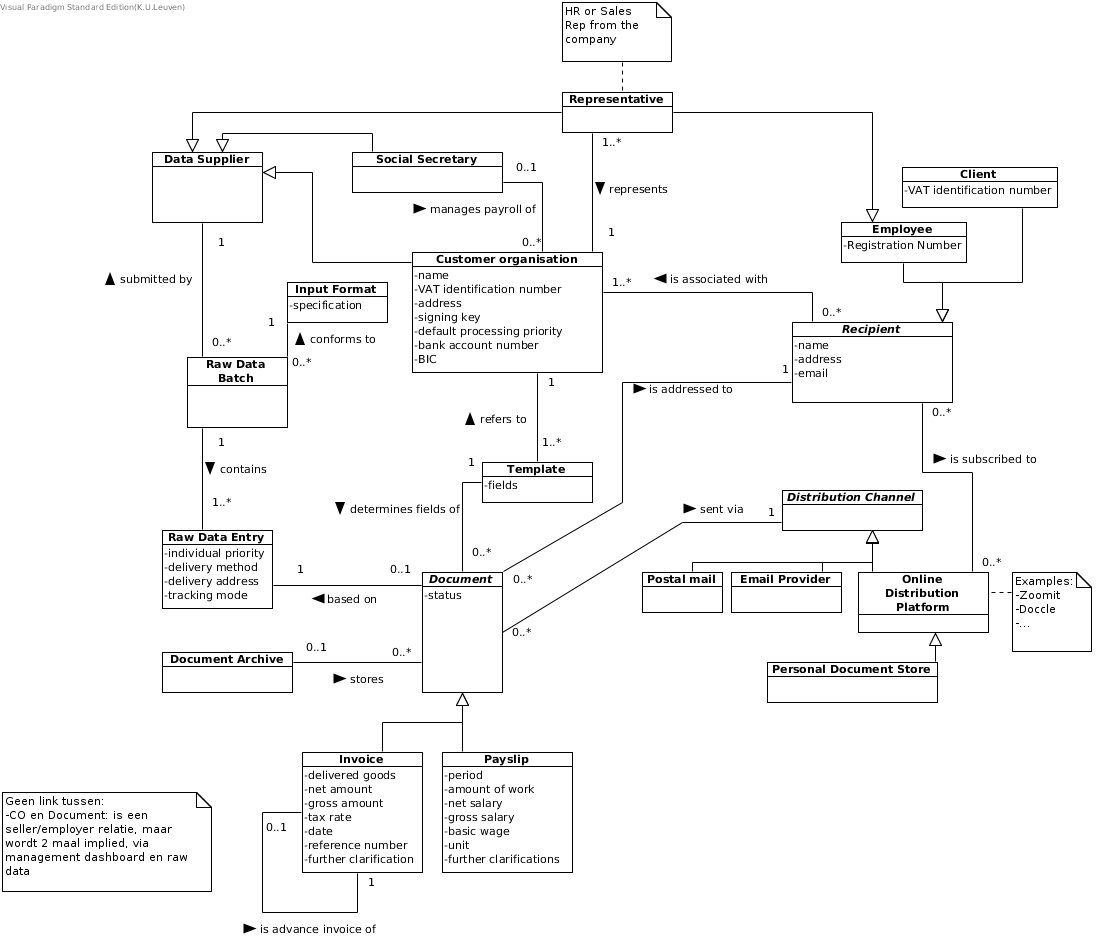
\includegraphics[width=0.8\textwidth]{domain_model.png}
    %\missingfigure[figwidth=0.8\textwidth]{Domain model}
    \caption{The domain model for the system.}\label{fig:domain_model}
\end{figure}

\subsection{Domain constraints}
In this section we provide additional domain constraints.

\begin{itemize}
    \item This is a first constraint.
    \item This is a second constraint.
\end{itemize}

\subsection{Glossary}
In this section, we provide a glossary of the most important terminology used
in this analysis.

\begin{itemize}
    \item \textbf{Term1}: definition
    \item \textbf{Term2}: definition
\end{itemize}

\section{Functional requirements}\label{sec:functional}
\subsection*{Use case model}

\begin{figure}[!htp]
    \centering
    %\includegraphics[width=0.8\textwidth]{}
    \missingfigure[figwidth=0.8\textwidth]{Use case model}
    \caption{Use case diagram for the system.}\label{fig:use_case_model}
\end{figure}

\subsection{\emph{UC7}: Filter documents in Personal Document Store}
\begin{itemize}
    \item \textbf{Primary actor:} Registered Recipient
    \item \textbf{Interested parties:} 
        \begin{itemize}
            \item \textit{eDocs:} Wants to know popular searches for optimising document caching
        \end{itemize}

    \item \textbf{Preconditions:}
        \begin{itemize}
            \item User has consulted his personal document store (UC4).
        \end{itemize}

    \item \textbf{Postconditions:}
        \begin{itemize}
            \item The Registered Recipient has received a new view of documents in his Personal document store, matching the query he gave to the system.
        \end{itemize}
        
    \item \textbf{Main scenario:} 
    \begin{enumerate}
       \item The user indicates he wants to pose a filter query to the Personal Document Store
       \item The user receives a form with filter choices, which he completes, and indicates he wants to filter with given parameters.
       \item The System retrieves all documents of the Registered User matching his query.
       \item The System provides an overview of all retrieved documents matching the User's query.
    \end{enumerate}

    \item \textbf{Alternative scenarios:} 
    \begin{enumerate}
        \item [4a.] The System did not find any documents matching the User's query
        \item [5a.] The Registered User receives a notification that no documents have matched his filter parameters.
    \end{enumerate}
    
    \item \textbf{Remarks:}
        \begin{itemize}
            \item Abstraction is made of the contents of the filter form. The given choices can be free form or very simple ones.
        \end{itemize}
\end{itemize}

\subsection{\emph{UC8}: Consult Document Delivery status}
\begin{itemize}
    \item \textbf{Primary actor:} Customer Organisation Representative
    \item \textbf{Interested parties:} 
        \begin{itemize}
            \item \textit{eDocs:} wants to let the organisation know their documents are actually being delivered
        \end{itemize}

    \item \textbf{Preconditions:}
        \begin{itemize}
            \item The Representative is logged in (UC1).
        \end{itemize}

    \item \textbf{Postconditions:}
        \begin{itemize}
            \item Representative has received Delivery information regarding the documents he is interested in.
        \end{itemize}
        
    \item \textbf{Main scenario:} 
    \begin{enumerate}
       \item The Representative signals he wants an overview of the company documents to which he has access (see remarks).
       \item The System retrieves all documents managed by the Representative.
       \item The System presents the Representative with an overview of the matching documents, including a small individual note per document whether it has been delivered or not.
       \item The use case ends here.
    \end{enumerate}

    \item \textbf{Alternative scenarios:} 
    \begin{enumerate}
        \item [4a.] The Representative indicates he wants to see details (see remarks) of a document present in the overview.
        \item [5a.] The System presents the Representative with the detailed information for indicated document.
        \item [4b.] The Representative indicates he only wants to see undelivered documents.
        \item [5b.] The System retrieves all undelivered documents managed by the Representative.
        \item [6b.] The System presents the Representative with an overview of the retrieved documents.
    \end{enumerate}
    
    \item \textbf{Remarks:}
        \begin{itemize}
            \item A representative only has access to documents generated by his role in the company. E.g. Sales representatives cannot consult payslips, which are managed by Human Resources Representatives.
            \item A document in an online distribution platform is only flagged as delivered after the document has also been opened by the Recipient.
            \item Details of a document in this Use Case denote for example the chosen distribution channel, the contents of the document, the date of generation \ldots
        \end{itemize}
\end{itemize}

\subsection{\emph{UC9}: Submit Raw Data}
\begin{itemize}
    \item \textbf{Primary actor:} Customer Organisation or Social Secretary
    \item \textbf{Interested parties:} 
        \begin{itemize}
            \item \textit{Customer Organisation Representative:} wants to make sure the documents he manages are correctly generated and delivered from the raw data
            \item \textit{eDocs:} wants the system to correctly handle raw data or signal the company if errors exist
        \end{itemize}

    \item \textbf{Preconditions:}
        \begin{itemize}
            \item The primary actor is authenticated (UC1).
        \end{itemize}

    \item \textbf{Postconditions:}
        \begin{itemize}
            \item The System has received a correct batch of data which can be processed into docuents.
            \item The Customer Organisation knows that no errors are present in the currently submitted data.
        \end{itemize}
        
    \item \textbf{Main scenario:} 
    \begin{enumerate}
       \item The primary actor submits over agreed protocol a batch of raw data for processing.
       \item The System verifies that the raw data entries are all correctly formatted.
       \item The Use Case ends here.
    \end{enumerate}

    \item \textbf{Alternative scenarios:} 
    \begin{enumerate}
        \item [3a.] The System finds one or more entries in the raw data which are not correctly formatted.
        \item [4a.] The System collects all incorrect entries.
        \item [5a.] The System sends a notice to the responsible Customer Organisation Representative(s) that errors have been found in recently submitted data.
    \end{enumerate}
    
    \item \textbf{Remarks:}
        \begin{itemize}
            \item The Customer Organisation as specified in the primary actors can mean a specific user periodically submitting data batches, but is mostly implied to be an automated system in the company, handling the batches of raw data. Analogous for the Social Secretary.
            \item Authentication of the primary actor can be through an interactive login procedure, but could also be automated authentication for the company systems, so they can automatically and periodically submit accumulated batches of raw data without user intervention.
        \end{itemize}
\end{itemize}

\subsection{\emph{UC10}: Handle Raw Data error}
\begin{itemize}
    \item \textbf{Primary actor:} Customer Organisation Representative
    \item \textbf{Interested parties:} 
        \begin{itemize}
            \item \textit{Customer Organisation:} wants to make sure its documents are correctly generated and delivered
            \item \textit{Social Secretary:} wants know if errors existed in the data they submitted, to check if their bookkeeping is sound.
        \end{itemize}

    \item \textbf{Preconditions:}
        \begin{itemize}
            \item The System has received a batch of raw data and found errors in the entries
            \item The System has sent a notice to the responsible Customer Organisation Representative.
            \item The Customer Organisation Representative as primary actor is responsible for the document type for which an error was present in the raw data.
        \end{itemize}

    \item \textbf{Postconditions:}
        \begin{itemize}
            \item The System has received new raw data to replace the data entries which contained errors.
            \item No new errors are present in the newly submitted raw data entries.
        \end{itemize}
        
    \item \textbf{Main scenario:} 
    \begin{enumerate}
       \item The Representative receives a notice that errors were present in a recently submitted raw data batch.
       \item The Representative logs in to the system (UC1).
       \item The Representative indicates he wants to receive an overview of the data errors to be handled by him/her.
       \item The System collects all raw data errors for which the Representative is responsible.
       \item The System presents the Representative with an overview of retrieved errors.
       \item the Representative gathers the correct data.
       \item The Representative submits over agreed protocol the new batch of raw data for processing.
       \item The System checks the new raw data for errors.
       \item No errors are found and the system indicates to the Representative that his submission was succesful.
    \end{enumerate}

    \item \textbf{Alternative scenarios:} 
    \begin{enumerate}
        \item [9a.] Errors are detected in the newly submitted data.
        \item [10a.] The System sends a notice to the responsible Customer Organisation Representative(s) that errors have been found in recently submitted data.
    \end{enumerate}
    
    \item \textbf{Remarks:}
        \begin{itemize}
            \item Abstraction is made of the way the Representative receives the notification. This could be by email or an external notification system of the company or eDocs. In this case the Log-In step is necessary. If the notice is internal to the eDocs system, and the Representative only receives it after logging in, the Log-In (UC1) step becomes a precondition.
            \item The agreed protocol for submission by the Representative should include a way to signal that the submitted raw data replaces erronous data. It could be a more interactive way of submitting data, for example, a field or button in the overview of the retrieved errors.
        \end{itemize}
\end{itemize}

\subsection{\emph{UC11}: Name of use case 11}
\begin{itemize}
    \item \textbf{Primary actor:} primary actor
    \item \textbf{Interested parties:} 
        \begin{itemize}
            \item \textit{Name of interested party:} reason why party is interested
        \end{itemize}

    \item \textbf{Preconditions:}
        \begin{itemize}
            \item First precondition.
            \item Second precondition.
        \end{itemize}

    \item \textbf{Postconditions:}
        \begin{itemize}
            \item First postcondition.
            \item Second postcondition.
        \end{itemize}
        
    \item \textbf{Main scenario:} 
    \begin{enumerate}
       \item Step 1
       \item Step 2
       \item Step 3
       \item \ldots
    \end{enumerate}

    \item \textbf{Alternative scenarios:} 
    \begin{enumerate}
        \item [3b.] Alternative at step 3
    \end{enumerate}
    
    \item \textbf{Remarks:}
        \begin{itemize}
            \item First remark
        \end{itemize}
\end{itemize}

\subsection{\emph{UC12}: Name of use case 12}
\begin{itemize}
    \item \textbf{Primary actor:} primary actor
    \item \textbf{Interested parties:} 
        \begin{itemize}
            \item \textit{Name of interested party:} reason why party is interested
        \end{itemize}

    \item \textbf{Preconditions:}
        \begin{itemize}
            \item First precondition.
            \item Second precondition.
        \end{itemize}

    \item \textbf{Postconditions:}
        \begin{itemize}
            \item First postcondition.
            \item Second postcondition.
        \end{itemize}
        
    \item \textbf{Main scenario:} 
    \begin{enumerate}
       \item Step 1
       \item Step 2
       \item Step 3
       \item \ldots
    \end{enumerate}

    \item \textbf{Alternative scenarios:} 
    \begin{enumerate}
        \item [3b.] Alternative at step 3
    \end{enumerate}
    
    \item \textbf{Remarks:}
        \begin{itemize}
            \item First remark
        \end{itemize}
\end{itemize}

\subsection{\emph{UC13}: Deliver generated document}
\begin{itemize}
    \item \textbf{Primary actor:} Recipient
    \item \textbf{Interested parties:} 
        \begin{itemize}
            \item \textit{eDocs:} wants documents to be delivered with as little human interaction as possible
            \item \textit{Customer Organization:} wants their documents to be delivered
        \end{itemize}

    \item \textbf{Preconditions:}
        \begin{itemize}
            \item Either the Customer Organisation or a Customer Organisation Representative has delivered a Data Batch containing the information necessary to generate the document.
            \item The document has been generated successfully.
        \end{itemize}

    \item \textbf{Postconditions:}
        \begin{itemize}
            \item The document has been sent on its way via the chosen Distribution Channel
        \end{itemize}
        
    \item \textbf{Main scenario:} 
    \begin{enumerate}
       \item The System selects a Distribution Channel specified by the raw data or according to information the System knows about the Recipient (see remark 1)
       \item If the document was not a part of an automatic Data Batch, the Customer Organisation is billed with the costs of sending the document
       \item The System marks the document as sent.
    \end{enumerate}

    \item \textbf{Alternative scenarios:} 
    None
    
    \item \textbf{Remarks:}
        \begin{itemize}
            \item Step 1 is an extension point for other use cases
        \end{itemize}
\end{itemize}

\subsection{\emph{UC14}: Deliver document via print \& postal service}
\begin{itemize}
    \item \textbf{Primary actor:} Recipient
    \item \textbf{Interested parties:} 
        \begin{itemize}
            \item \textit{Print \& postal service:} provides delivery of traditional mail
        \end{itemize}

    \item \textbf{Preconditions:}
        \begin{itemize}
            \item The document's associated raw data specifies print \& postal service as the delivery method
            \item It is not the case that the System knows that the Recipient is registered with an Online Distribution Platform that distributes the type of the document to be delivered.
        \end{itemize}

    \item \textbf{Postconditions:}
        \begin{itemize}
            \item The System has sent a PDF representing the document to the print \& postal service via a web service.
        \end{itemize}
        
    \item \textbf{Main scenario:} 
    \begin{enumerate}
       \item The System retrieves the Recipient's postal address from the raw data.
       \item The System sends the PDF representing the document to the print \& postal service via a web service, along with the Recipient's postal address.
    \end{enumerate}

    \item \textbf{Alternative scenarios:} 
    None
    
    \item \textbf{Remarks:}
        \begin{itemize}
            \item This use case is an extension of UC13: Deliver generated document
        \end{itemize}
\end{itemize}

\subsection{\emph{UC15}: Deliver document via e-mail}
\begin{itemize}
    \item \textbf{Primary actor:} Unregistered Recipient
    \item \textbf{Interested parties:} 
        \begin{itemize}
            \item \textit{E-mail Provider:} Is responsible for delivering e-mail addressed to its clients
        \end{itemize}

    \item \textbf{Preconditions:}
        \begin{itemize}
            \item It is not the case that the System knows that the Recipient is registered with an Online Distribution Platform that distributes the type of the document to be delivered.
        \end{itemize}

    \item \textbf{Postconditions:}
        \begin{itemize}
            \item The System has sent an e-mail to the Recipient with PDF representing the document included as an attachment
        \end{itemize}
        
    \item \textbf{Main scenario:} 
    \begin{enumerate}
       \item The System retrieves the Recipient's e-mail address from the document's raw data.
       \item The System composes an e-mail and includes the PDF representing the document as an attachment
       \item The System sends the e-mail on its way
    \end{enumerate}

    \item \textbf{Alternative scenarios:} 
    \begin{enumerate}
        \item [2a.] If receipt tracking is enabled, the System composes an e-mail consisting of a short description of the document and a unique URL providing access to the document.
        \item [3a.] The System sends the e-mail on its way
        \item [4a.] The System arranges for an event to be fired that marks delivery failure should the Recipient not have followed the link within 30 days
    \end{enumerate}
    
    \item \textbf{Remarks:}
        \begin{itemize}
            \item This use case is an extension of UC13: Deliver generated document
        \end{itemize}
\end{itemize}

\subsection{\emph{UC16}: Deliver document via Online Distribution Platform}
\begin{itemize}
    \item \textbf{Primary actor:} Recipient
    \item \textbf{Interested parties:} 
        \begin{itemize}
            \item \textit{Online Distribution Platform:} wants to deliver documents addressed to its clients
        \end{itemize}

    \item \textbf{Preconditions:}
        \begin{itemize}
            \item The System knows that the Recipient is registered with an Online Distribution Platform that distributes the type of the document to be delivered
        \end{itemize}

    \item \textbf{Postconditions:}
        \begin{itemize}
            \item The System has sent the PDF representing the document to the Online Distribution Platform via a web service along with information
            that identifies the Recipient
        \end{itemize}
        
    \item \textbf{Main scenario:} 
    \begin{enumerate}
       \item The System retrieves information that identifies the Recipient from the document's raw data
       \item The System sends the PDF representing the information and the identifying information via a web service to the Online Distribution Platform
       \item If the Customer Organization has requested receipt tracking and if the Online Distribution Platform supports it, the System indicates this to the Online Distribution Platform
    \end{enumerate}

    \item \textbf{Alternative scenarios:} 
    None
    
    \item \textbf{Remarks:}
        \begin{itemize}
          \item  This use case is an extension of UC13: Deliver generated document
        \end{itemize}
\end{itemize}

\subsection{\emph{UC17}: Consult Billing Information}
\begin{itemize}
	\item \textbf{Primary actor:} Customer Organization
	\item \textbf{Interested parties:} 
	\begin{itemize}
		\item \textit{eDocs:} wants to store all information concerning financial transactions
		\item \textit{Social Secretary:} wants to know the costs it has incurred on behalf of the Customer Organization
	\end{itemize}
	
	\item \textbf{Preconditions:}
	\begin{itemize}
		\item The user is logged in (UC1: Log in)
	\end{itemize}
	
	\item \textbf{Postconditions:}
	\begin{itemize}
		\item The System has presented the user with an overview of billing information
	\end{itemize}
	
	\item \textbf{Main scenario:} 
	\begin{enumerate}
		\item The user indicates he wishes to view the Customer Organization's billing information
		\item The System collects the Customer Organization's billing information
		\item The System presents the user with an overview of the retrieved billing information
		\item The use case ends
	\end{enumerate}
	
	\item \textbf{Alternative scenarios:} 
	\begin{enumerate}
		\item [4a.] The user indicates that he wants a more detailed view of a specific transaction
		\item [5a.] The System presents the user with a more detailed view of that transaction
		\item [6a.] The user indicates he wants to return to the overview
		\item [7a.] The use case goes back to step 3
	\end{enumerate}
	
	\item \textbf{Remarks:}
	None
\end{itemize}

\subsection{\emph{UC18}: Manage Customer Organization information}
\begin{itemize}
	\item \textbf{Primary actor:} eDocs System Administrator
	\item \textbf{Interested parties:} 
	\begin{itemize}
		\item \textit{Customer Organization:} desires an adequate level of service from eDocs
	\end{itemize}
	
	\item \textbf{Preconditions:}
	\begin{itemize}
		\item The Customer Organization has been registered with the System
		\item The eDocs System Administrator is logged in (UC1: Log in)
	\end{itemize}
	
	\item \textbf{Postconditions:}
	\begin{itemize}
		\item Any changes made by the eDocs System Administrator have been logged
	\end{itemize}
	
	\item \textbf{Main scenario:} 
	\begin{enumerate}
		\item The Administrator indicates he wants to view the Customer Organization's information stored by the System
		\item The System presents an overview of the Customer Organization's information
		\item The use case ends
	\end{enumerate}
	
	\item \textbf{Alternative scenarios:} 
	\begin{enumerate}
		\item [3a.] The Administrator indicates he wants to edit the Customer Organization's information (e.g. the Service Level Agreement has been revised and any changes need to be logged)
		\item [4a.] The System provides the Administrator with the means to edit the relevant information
		\item [5a.] The Administrator indicates he has finished editing the information
		\item [6a.] The use case goes back to step 2
	\end{enumerate}
	
	\item \textbf{Remarks:}
	\begin{itemize}
		\item First remark
	\end{itemize}
\end{itemize}

\subsection{\emph{UC19}: Register Customer Organization}
\begin{itemize}
	\item \textbf{Primary actor:} eDocs System Administrator
	\item \textbf{Interested parties:} 
	\begin{itemize}
		\item \textit{eDocs:} wants as many clients to use their services as possible
		\item \textit{Customer Organization:} wants to use eDocs's services and is prepared to provide monetary compensation
	\end{itemize}
	
	\item \textbf{Preconditions:}
	\begin{itemize}
		\item Negotiations regarding the Service Level Agreement were successful
		\item The eDocs System Administrator is logged in (UC1: Log in)
	\end{itemize}
	
	\item \textbf{Postconditions:}
	\begin{itemize}
		\item An account for the Customer Organization has been opened in addition to accounts for any representatives, if applicable
	\end{itemize}
	
	\item \textbf{Main scenario:} 
	\begin{enumerate}
		\item The eDocs System Administrator indicates he wants to register a new Customer Organization
		\item The System provides the Administrator with the means to input the required information (e.g. default priority level, credentials for any automatic data delivery channels, etc.)
		\item The Administrator inputs the required information
		\item The Administrator indicates he has finished providing the information
		\item The System creates an account on behalf of the Customer Organization and any representatives, if applicable
		\item The use case ends
	\end{enumerate}
	
	\item \textbf{Alternative scenarios:} 
	\begin{enumerate}
		\item [5a.] The System indicates that the information provided was incomplete or invalid
		\item [6a.] The use case goes back to step 3
	\end{enumerate}
	
	\item \textbf{Remarks:}
	\begin{itemize}
		\item First remark
	\end{itemize}
\end{itemize}

\subsection{\emph{UC20}: Unregister Customer Organization}
\begin{itemize}
	\item \textbf{Primary actor:} eDocs System Administrator
	\item \textbf{Interested parties:} 
	\begin{itemize}
		\item \textit{eDocs:} wishes to have an accurate view of their client base
		\item \textit{Customer Organization:} no longer wants to be serviced by eDocs
	\end{itemize}
	
	\item \textbf{Preconditions:}
	\begin{itemize}
		\item The Customer Organization has been registered
		\item The Customer Organization has authorized account removal
		\item The eDocs System Administrator is logged in (UC1: Log in)
		\item The eDocs System Administrator has consulted the Customer Organization's information (UC18: Manage Customer Organization Information)
	\end{itemize}
	
	\item \textbf{Postconditions:}
	\begin{itemize}
		\item All accounts associated with the Customer Organization have been removed. Any documents generated on the Customer Organization's behalf remain untouched.
	\end{itemize}
	
	\item \textbf{Main scenario:} 
	\begin{enumerate}
		\item The eDocs System Administrator indicates he wishes to unregister the Customer Organization
		\item The System removes all accounts associated with the Customer Organization
	\end{enumerate}
	
	\item \textbf{Alternative scenarios:} 
	None
	
	\item \textbf{Remarks:}
	None
\end{itemize}

\subsection{\emph{UC21}: Register Recipient association with Online Distribution Platform}
\begin{itemize}
	\item \textbf{Primary actor:} Online Distribution Platform
	\item \textbf{Interested parties:} 
	\begin{itemize}
		\item \textit{eDocs:} wishes to comply to the Recipient's preferences as to how he wants his documents to be delivered
		\item \textit{Recipient:} wants documents addressed to him to be delivered according to his wishes
	\end{itemize}
	
	\item \textbf{Preconditions:}
	None
	
	\item \textbf{Postconditions:}
	\begin{itemize}
		\item The System now sends documents addressed to the Recipient of the types that the Online Distribution Platform distributes to the Online Distribution Platform
	\end{itemize}
	
	\item \textbf{Main scenario:} 
	\begin{enumerate}
		\item The Online Distribution Platform indicates that the Recipient wishes to receive documents through them
		\item The Online Distribution Platform supplies identifying information pertaining to the Recipient
		\item The System logs that any documents addressed to the Recipient of the types that the Online Distribution Platform distributes are to be sent to the Online Distribution Platform
		\item The use case ends
	\end{enumerate}
	
	\item \textbf{Alternative scenarios:} 
	\begin{enumerate}
		\item [3a.] The System has determined that the identifying information does not allow the Recipient to be successfully identified (e.g. the Online Distribution Platform distributes invoices and the bank account number was not formatted correctly or no bank account number was supplied at all)
		\item [4a.] This anomaly is logged for review by an eDocs System Administrator
		\item [5a.] The use case ends
	\end{enumerate}
	
	\item \textbf{Remarks:}
	None
\end{itemize}

\subsection{\emph{UC22}: Register Recipient unregistration with Online Distribution Platform}
\begin{itemize}
	\item \textbf{Primary actor:} Online Distribution Platform
	\item \textbf{Interested parties:} 
	\begin{itemize}
		\item \textit{eDocs:} wishes to comply to the Recipient's preferences as to how he wants his documents to be delivered
		\item \textit{Recipient:} wants documents addressed to him to be delivered according to his wishes
	\end{itemize}
	
	\item \textbf{Preconditions:}
	\begin{itemize}
		\item The Recipient has been registered as associated with the Online Distribution Platform
	\end{itemize}
	
	\item \textbf{Postconditions:}
	\begin{itemize}
		\item The System has logged that any overrides pertaining to document types distributed by the Online Distribution Platform no longer apply in the Recipient's case
	\end{itemize}
	
	\item \textbf{Main scenario:} 
	\begin{enumerate}
		\item The Online Distribution Platform has indicated that they no longer service the Recipient
		\item The Online Distribution Platform supplies identifying information pertaining to the Recipient
		\item The System removes any overrides pertaining to document types distributed by the Online Distribution Platform
		\item The use case ends
	\end{enumerate}
	
	\item \textbf{Alternative scenarios:} 
	\begin{enumerate}
		\item [3a.] The System has determined that the identifying information fails to successfully identify the Recipient
		\item [4a.] This anomaly is logged for review by an eDocs System Administrator
		\item [5a.] The use case ends
	\end{enumerate}
	
	\item \textbf{Remarks:}
	\begin{itemize}
		\item First remark
	\end{itemize}
\end{itemize}

\subsection{\emph{UC23}: Confirm delivery through receipt tracking}
\begin{itemize}
	\item \textbf{Primary actor:} Recipient
	\item \textbf{Interested parties:} 
	\begin{itemize}
		\item \textit{eDocs:} wishes to assure the Company Organization that their documents are being delivered
		\item \textit{Customer Organization:} wishes to be certain that documents sent on their behalf have been delivered
	\end{itemize}
	
	\item \textbf{Preconditions:}
	\begin{itemize}
		\item Receipt tracking was activated for the delivered document
	\end{itemize}
	
	\item \textbf{Postconditions:}
	\begin{itemize}
		\item The System has marked the document as delivered
	\end{itemize}
	
	\item \textbf{Main scenario:} 
	\begin{enumerate}
		\item The Recipient triggers receipt confirmation (see remark 1)
		\item The System marks the relevant document as delivered
	\end{enumerate}
	
	\item \textbf{Alternative scenarios:} 
	None
	
	\item \textbf{Remarks:}
	\begin{itemize}
		\item Step 1 is an extension point for other use cases
	\end{itemize}
\end{itemize}

\subsection{\emph{UC24}: Confirm delivery through e-mail receipt tracking}
\begin{itemize}
	\item \textbf{Primary actor:} Recipient
	\item \textbf{Interested parties:} 
	\begin{itemize}
		\item \textit{eDocs:} wishes to assure the Company Organization that their documents are being delivered
		\item \textit{Customer Organization:} wishes to be certain that documents sent on their behalf have been delivered
	\end{itemize}
	
	\item \textbf{Preconditions:}
	\begin{itemize}
		\item The document was sent by e-mail
	\end{itemize}
	
	\item \textbf{Postconditions:}
	\begin{itemize}
		\item The System has marked the document as delivered
	\end{itemize}
	
	\item \textbf{Main scenario:} 
	\begin{enumerate}
		\item The Recipient follows the unique URL provided in the e-mail
		\item The System registers that the Recipient has followed the URL
	\end{enumerate}
	
	\item \textbf{Alternative scenarios:} 
	\begin{enumerate}
		\item [2a.] The System has previously perceived that the Recipient did not follow the URL within 30 days of the System sending the document and therefore does not respond to the Recipient following the link beyond indicating that the URL is no longer valid
		\item [3a.] The use case ends
	\end{enumerate}
	
	\item \textbf{Remarks:}
	\begin{itemize}
		\item This use case is an extension of UC23: Confirm delivery through receipt tracking
	\end{itemize}
\end{itemize}

\subsection{\emph{UC25}: Confirm delivery through Online Distribution Service receipt tracking}
\begin{itemize}
	\item \textbf{Primary actor:} Online Distribution Platform
	\item \textbf{Interested parties:} 
	\begin{itemize}
		\item \textit{eDocs:} wishes to assure the Company Organization that their documents are being delivered
		\item \textit{Customer Organization:} wishes to be certain that documents sent on their behalf have been delivered
	\end{itemize}
	
	\item \textbf{Preconditions:}
	\begin{itemize}
		\item Receipt tracking has been requested by the Customer Organization
		\item The Online Distribution Platform supports receipt tracking
	\end{itemize}
	
	\item \textbf{Postconditions:}
	\begin{itemize}
		\item The System has marked the document as delivered
	\end{itemize}
	
	\item \textbf{Main scenario:} 
	\begin{enumerate}
		\item The Online Distribution platform indicates that the Recipient has received the document
	\end{enumerate}
	
	\item \textbf{Alternative scenarios:} 
	None
	
	\item \textbf{Remarks:}
	\begin{itemize}
		\item This use case is an extension of UC23: Confirm delivery through receipt tracking
	\end{itemize}
\end{itemize}

\section{Non-functional requirements}\label{sec:non-functional}
In this section, we model the non-functional requirements for the system in the
form of \emph{quality attribute scenarios}. We provide for each type
(availability, performance and modifiability) one requirement.

\subsection{Availability}
\subsubsection{\emph{Av1}: Name of the quality attribute scenario}
Shortly describe the context of the scenario.

\begin{itemize}
    \item \textbf{Source:} source
    \item \textbf{Stimulus:}
        \begin{itemize}
            \item Description of a first stimulus.
            \item Description of a second stimulus.
        \end{itemize}

    \item \textbf{Artifact:} the stimulated artifact
    \item \textbf{Environment:} the condition under which the stimulus occurs
    \item \textbf{Response:}
        \begin{itemize}
            \item Describe how the system should respond to the stimulus.
        \end{itemize}

    \item \textbf{Response measure:}
        \begin{itemize}
            \item Describe how the satisfaction of a response is measured.
        \end{itemize}
\end{itemize}

\subsection{Performance}
\subsubsection{\emph{P1}: Name of the quality attribute scenario}
Shortly describe the context of the scenario.

\begin{itemize}
    \item \textbf{Source:} source
    \item \textbf{Stimulus:}
        \begin{itemize}
            \item Description of a first stimulus.
            \item Description of a second stimulus.
        \end{itemize}

    \item \textbf{Artifact:} the stimulated artifact
    \item \textbf{Environment:} the condition under which the stimulus occurs
    \item \textbf{Response:}
        \begin{itemize}
            \item Describe how the system should respond to the stimulus.
        \end{itemize}

    \item \textbf{Response measure:}
        \begin{itemize}
            \item Describe how the satisfaction of a response is measured.
        \end{itemize}
\end{itemize}

\subsection{Modifiability}
\subsubsection{\emph{M1}: Name of the quality attribute scenario}
Shortly describe the context of the scenario.

\begin{itemize}
    \item \textbf{Source:} source
    \item \textbf{Stimulus:}
        \begin{itemize}
            \item Description of a first stimulus.
            \item Description of a second stimulus.
        \end{itemize}

    \item \textbf{Artifact:} the stimulated artifact
    \item \textbf{Environment:} the condition under which the stimulus occurs
    \item \textbf{Response:}
        \begin{itemize}
            \item Describe how the system should respond to the stimulus.
        \end{itemize}

    \item \textbf{Response measure:}
        \begin{itemize}
            \item Describe how the satisfaction of a response is measured.
        \end{itemize}
\end{itemize}

\end{document}
